\section{Der SMD-Assistent im GDS-System} \label{SMD-Assistent}
Die \ac{SMD} enthalten alle wichtigen Informationen um die Struktur einer Klasse zu beschreiben. Diese Klasseninformationen sollen sp\"ater von einem SMD-Assistenten verwaltet werden.

Die \ac{SMD}-grundlegenden Informationen wie Klassenname, Methodennamen und Attributnamen, aber auch Attribut-Qualifier und -Modifier, sowie Methoden-Qualifier, -Modifier und Parameterlisten der Methoden, sind vorhanden.
Zus\"atzlich ist gespeichert, von welcher Klasse geerbt wird, beziehungsweise welche implementiert wurden.

In einer MySQL-Datenbank k\"onnen alle eben genannten Klasseninformationen gespeichert werden. Zus\"atzlich werden in der Datenbank Referenzen zu Klassen aufgebaut, von welchen geerbt beziehungsweise welche implementiert wurden.
Au\ss{}erdem werden Klassenattribute in der Datenbank referenziert. \cite{Zil14}

Da es sich bei den \ac{SMD} um reine Metadaten handelt, werden keine Methodenr\"umpfe in die \ac{SMD}-Datenbank aufgenommen.

Der Nutzer des \ac{GDS}-Systems gibt \"uber den \ac{UDDE}, also das User Interface, seine Klassen und \ac{AMD} in das System. Er kann \"uber den \ac{UDDE} ein komplettes "`Klassengr\"ust"', also alle \ac{SMD} erstellen, indem er alle Klassenattribute und Methoden angibt, sowie referenzierte Klassen angibt. 

Hierbei ist er nat\"urlich auch in der Lage den Modifier und den R\"uckgabetyp zu bestimmen. Bei Methoden k\"onnen nat\"urlich zus\"atzlich Parameterlisten angegeben werden.

Des Weiteren legt der \ac{UDDE} die generierten "`strukturellen Metadaten"', mit Hilfe des \ac{SMD}-Assistenten in einer Datenbank ab, welche sp\"ater vom SMD-Assistenten auch wieder ausgelesen werden k\"onnen.

Der SMD-Assistent ist f\"ur das Umwandeln von Klassen in \ac{SMD} verantwortlich. Nach dem Erstellen der \ac{SMD} werden diese zur Aufbewahrung vom Assistenten in einer Datenbank verwaltet.

Die \ac{SMD} werden von der Anwendung an verschiedenen Stellen ben\"otigt, so zum Beispiel beim Serialisieren. Ein \ac{CG} wandelt die \ac{SMD} wieder in Programmcode, welcher \ac{OPM}-konform erzeugt wird. Eine genaue Spezifikation f\"ur den Klassengenerator ist im Kapitel \ref{CG} zu finden.
Die generierten Daten k\"onnen dann ebenfalls vom \ac{GDS} in einer Datenbank gespeichert werden.

Der \ac{IG} erstellt aus den vom SMD-Assistenten gelieferten \ac{SMD} Schemata f\"ur \ac{JSON} und XML. Eine Funktion zur Erstellung des \ac{JSON}-Schemas aus einer Klasse wird in Kapitel \ref{JSON-Schema} beschrieben.
Auch das entsprechende Klassenschema soll vom \ac{GDS} in einer Datenbank abgelegt werden.

Der beschriebene Zusammenhang der Komponenten des \ac{GDS} ist im Bild auf der n\"achsten Seite noch einmal verdeutlicht.

\begin{figure}[!ht]
\centering
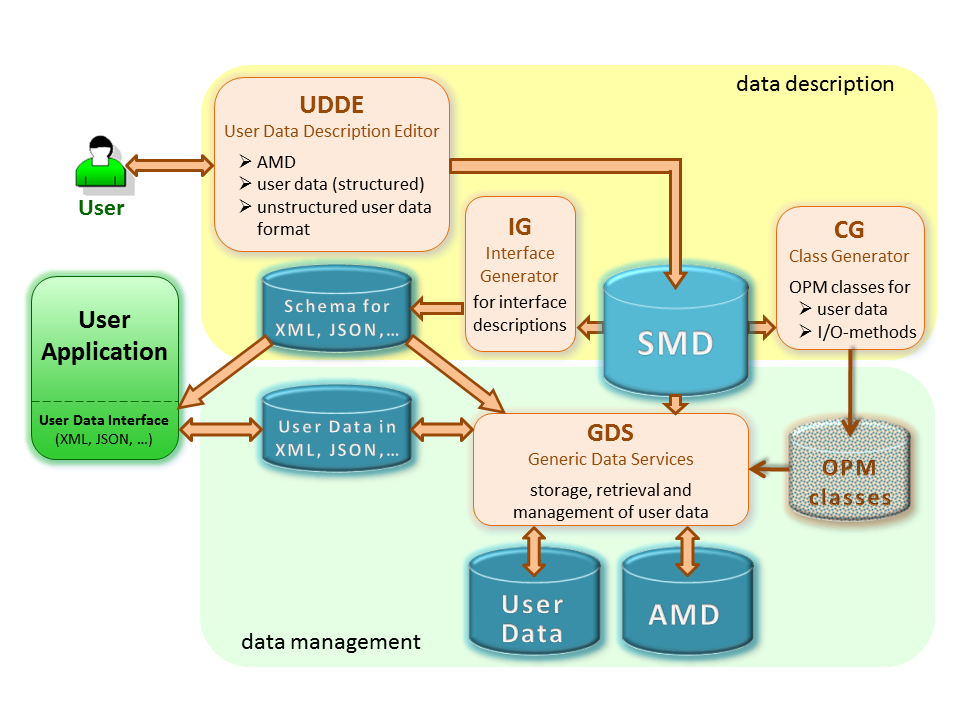
\includegraphics[width=13.5cm]{Bilder/UebersichtGDS}
\label{GDS \"Ubersicht}
\caption{GDS \"Ubersicht}
\centering
\end{figure}

\FloatBarrier

\subsection{Spezifikation des SMD-Assistenten}
Im Verlauf der Arbeit wurde zunehmend klar, dass die Spezifikation des SMD-Assistenten n\"otig wird, da die \ac{SMD}, wie im Schaubild oben zu erkennen, zentraler Bestandteil des Projektes sind.
Der SMD-Assistent wurde im Projekt \"ofter diskutiert und seine Funktionsweise soll an dieser Stelle einmal genauer erl\"autert werden.

\subsubsection{Funktionen des SMD-Assistenten}
Der SMD-Assistent soll die "`strukturellen Metadaten"' aus der Datenbank laden und diese an das \ac{GDS}, den \ac{IG} oder den \ac{CG} weiterreichen. Somit ruft jede Instanz, welche die \ac{SMD} ben\"otigt, den \ac{SMD}-Assistenten auf, damit dieser die ben\"otigten Informationen liefern kann.

Zu einer \texttt{ObjectID}, einer \texttt{ClassID} oder einem Klassennamen m\"ussen die passenden Metadaten aus der Datenbank geladen werden.
Die geladenen Daten werden in einer Instanz der Klasse \texttt{ClassDecr} zusammengefasst und mittels dieser Instanz \"ubergeben.

Objekte, welche serialisiert werden k\"onnen, haben eine \texttt{ObjectID}, anhand welcher sie eindeutig identifiziert werden k\"onnen. Zus\"atzlich k\"onnen \"uber die \texttt{ObjectID} auch verschiedene Instanzen eines Objektes unterschieden und zugeordnet werden. Dies geschieht \"uber die in der \texttt{ObjectID} vorhandene \texttt{InstanzID}.

Mittels einer \texttt{ClassID} k\"onnen genau wie mit der \texttt{ObjectID} Objekte identifiziert werden, jedoch keine bestimmten Instanzen.

Eine Instanz der Klasse \texttt{ClassDecr} enth\"alt mittels der Klassen \texttt{MethodDescr} und \texttt{AttrDecr} alle n\"otigen Informationen, um eine Klasse rekonstruieren zu k\"onnen. Sie stellen die "`strukturellen Metadaten"' dar.

\texttt{MethodDescr} enth\"alt eine Methode der Klasse, mit einer Liste von allen Parametern und deren Typen.
Die Klasse \texttt{AttrDecr} hingegen h\"alt jeweils ein Attribut mit dessen Informationen wie zum Beispiel Typ und Modifier. \cite{Zil14}

Der Zusammenhang ist im Klassendiagramm der SMD-Klassen noch einmal dargestellt. Im Bild 3, auf der n\"achsten Seite, ist aus Gr\"unden der \"Ubersichtlichkeit nicht der gesamte OPM-Klassenbaum abgebildet, sondern lediglich die f\"ur den \ac{SMD}-Assistent wichtigen Klassen sind aufgef\"uhrt.

Einmal aus der Datenbank geladene \ac{SMD} soll der SMD-Assistent zwischenspeichern, um beim erneuten Abfragen schneller reagieren zu k\"onnen. 

Damit es nicht zu einem Arbeitsspeicher\"uberlauf kommt, muss der SMD-Assistent genau wie zuk\"unftige andere Assistenten auch eine M\"oglichkeit besitzen, seinen internen Cache zu verkleinern. Dies soll \"uber einen m\"oglichst effizienten Scheduling-Algorithmus geschehen, welcher implementiert und auf Effizienz gepr\"uft werden muss.

Hier kommt ein weiterer Assistent zum Einsatz, und zwar der Speicher-Assistent, welcher bei geringem Arbeitsspeicher einen Befehl an alle Assistenten schickt, damit diese ihren Speicherbedarf reduzieren. Durch die Serialisierer wurde die \"Uberlegung zum Speicher-Assistenten zum ersten Mal entfacht, da hier teilweise sehr viel Arbeitsspeicher ben\"otigt wird. Dazu aber im n\"achsten Kapitel mehr.

\begin{figure}[!ht]
\centering
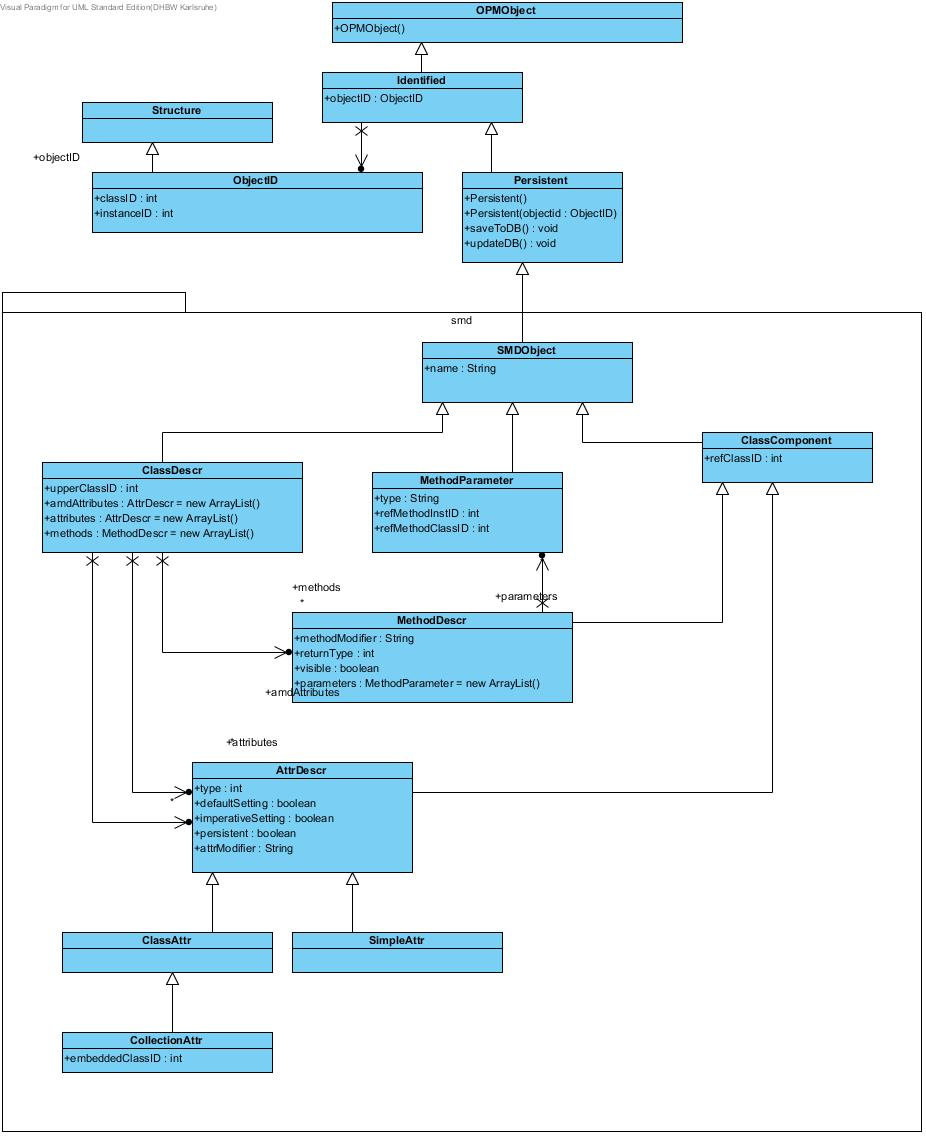
\includegraphics[width=13cm]{Bilder/SMD_Klassen}
\title{Klassendiagramm der SMD-Klassen}
\caption{Klassendiagramm der SMD-Klassen}
\centering
\end{figure}

\subsubsection{Der SMD-Assistent unter Java}
Unter Java kann die Arbeitsweise des SMD-Assistent deutlich vereinfacht werden, da hier die \ac{SMD} nur bei explizitem Verlangen geliefert werden m\"ussen, denn Java verwendet mit den \textit{.class}-Objekten eigene Metadaten, \"uber die eine Verarbeitung unter Java einfacher umgesetzt werden kann. 
Der SMD-Assistent sollte unter Java in der Lage, sein direkt Klassenobjekte zu liefern, da sich diese schneller verarbeiten lassen als die \ac{SMD}-Daten.

\subsection{Der Klassengenerator} \label{CG}
Der Klassengenerator ist ein Modul des \ac{GDS}, welches aus den vom \ac{SMD}-Assistenten gegebenen strukturellen Metadaten wieder Programmcode generiert. Es soll eine abstrakte Klasse \texttt{ClassGenerator} geben, welche abstrakte Methoden, zum Bauen einer Klasse, zur Verf\"ugung stellt. 

F\"ur jede Programmiersprache, soll nun ein Klassengenerator von der abstrakten Oberklasse abgeleitet werden. Die programmiersprachenspezifischen Klassengeneratoren sind dann in der Lage, f\"ur ihre Programmiersprache, aus den \ac{SMD}, Klassen zu generieren.

Da die Serialisierer wie Jackson und JAXB f\"ur Attribute, die nicht \texttt{public} sind, Getter- und Setter-Methoden ben\"otigen, muss der Klassengenerator diese erzeugen, auch wenn diese nicht in den \ac{SMD} auftauchen. Des Weiteren muss er diese Methoden auch nach dem OPM-Standard implementieren. Dies bedeutet, das in Setter-Methoden die Attribute gesetzt und in Getter-Methoden die Attribute gelesen werden m\"ussen.

Au\ss{}erdem ben\"otigen die Serialisierer auch Standardkonstruktoren, um ein leeres Element zu erstellen, welches im Laufe der Deserialisierung gef\"ullt werden kann.

Um die Serialisierer steuern zu k\"onnen, sind gegebenenfalls Annotations an den Klassen notwendig, welche ebenfalls vom \texttt{ClassGenerator} angebracht werden m\"ussen. Eine andere M\"oglichkeit w\"are, wie schon im Kapitel \ref{SMDAnnotationInsector} erw\"ahnt, die Verwendung der \ac{SMD} als Annotationsersatz.



